
%$$$$$$$$$$$$$$$$$$$$$$$$$$$$$$$$$$$$$$$$$$$$$$$$$$$$$$$$$$$$$$$$$$$$$$$$$$$$$$$$
%Paragraph 3: Scalable Data Structure and Lock에 대한 연구
%$$$$$$$$$$$$$$$$$$$$$$$$$$$$$$$$$$$$$$$$$$$$$$$$$$$$$$$$$$$$$$$$$$$$$$$$$$$$$$$$
\newpage
\section{확장성 있는 락 연구}
\label{sec:lockrelated}
%Scalable locks have been designed by the
%queue-based locks~\cite{MellorCrummey1991MCS}~\cite{Magnusson1994QLC},
%~\cite{Wang2016BeMyGuest},
%~\cite{Scott2013SS}
%~\cite{Bueso2014MCS}~\cite{Bueso2015STP}
%hierarchical locks~\cite{Radovic2003HBL}~\cite{Chabbi2016CLL} and
%~\cite{Luchangco2006HCQ}
%~\cite{Chabbi2015HPL}
%delegation
% techniques~\cite{Hendler2010FC}~\cite{Fatourou2012RCS}~\cite{Delegation2014}.

%Scalable locks have been designed by the
%queue-based locks~\cite{MellorCrummey1991MCS}~\cite{Magnusson1994QLC},
%~\cite{Wang2016BeMyGuest},
%~\cite{Scott2013SS}
%~\cite{Bueso2014MCS}~\cite{Bueso2015STP}
%hierarchical locks~\cite{Radovic2003HBL}~\cite{Chabbi2016CLL} and
%~\cite{Luchangco2006HCQ}
%~\cite{Chabbi2015HPL}
% delegation
%techniques~\cite{Hendler2010FC}~\cite{Fatourou2012RCS}~\cite{Delegation2014}.
확장성 있는 락들은 큐 기반의 락~\cite{MellorCrummey1991MCS}~\cite{Magnusson1994QLC},
~\cite{Wang2016BeMyGuest},
~\cite{Scott2013SS}
~\cite{Bueso2014MCS}~\cite{Bueso2015STP}과 계층적 락~\cite{Radovic2003HBL}~\cite{Chabbi2016CLL} and
~\cite{Luchangco2006HCQ}
~\cite{Chabbi2015HPL} 그리고 위임하는 방법(delegation
techniques)~\cite{Hendler2010FC}~\cite{Fatourou2012RCS}~\cite{Delegation2014}을 사용한다.

%Some approaches have been gradually adapted in real production software.
%For example, Linux kernel has replaced non-scalable locks with
%MCS locks~\cite{overviewofkernellock}.
%Our research is similar to the delegation techniques because
%the \LDU's \code{synchronize} function runs as a
%combiner thread;it improves cache locality.

\subsection{큐 기반의 락(Queued Lock)}


\subsubsection{MCS}



\subsection{계층적 락}

이 중 우리의 연구는 LDU의 \code{synchronize} 함수가 마치 FC의 컴파이너 쓰레드(combiner thread)와 같이
동작함으로 위임하는 방법과 비슷하다. 이것은 캐시의 지역성을 높이는 방법이다.
%However, our approach not only can improve cache locality but also
%can eliminate synchronization methods during updates due to using a lock-free
% manner.
하지만, 우리의 방법은 캐시의 지역성을 높일 뿐만아니라 업데이트 명령을
 수행하는 동안 락 프리(lock-free) 방법으로 동기화 기법들을 제거 할 수 있다. 
%MCS~\cite{MellorCrummey91}, a scalable lock.
%, is used in the Linux
%.
%In read-mostly data structures, RCU~\cite{McKenney98} can be quite useful.
%However, 
\subsubsection{HBL}



\subsubsection{CLL}


\subsubsection{HCQ}



\subsection{Delegation techniques}

\subsubsection{Flat Combining}



\subsubsection{OpLog}

OpLog는 RCU와 반대로 업데이트 비율이 높은 업데이트 헤비(Update heavy)한 자료구조를 위해 만든 
동기화 기법 중 하나이다.


\begin{figure}[h]
    \centering
    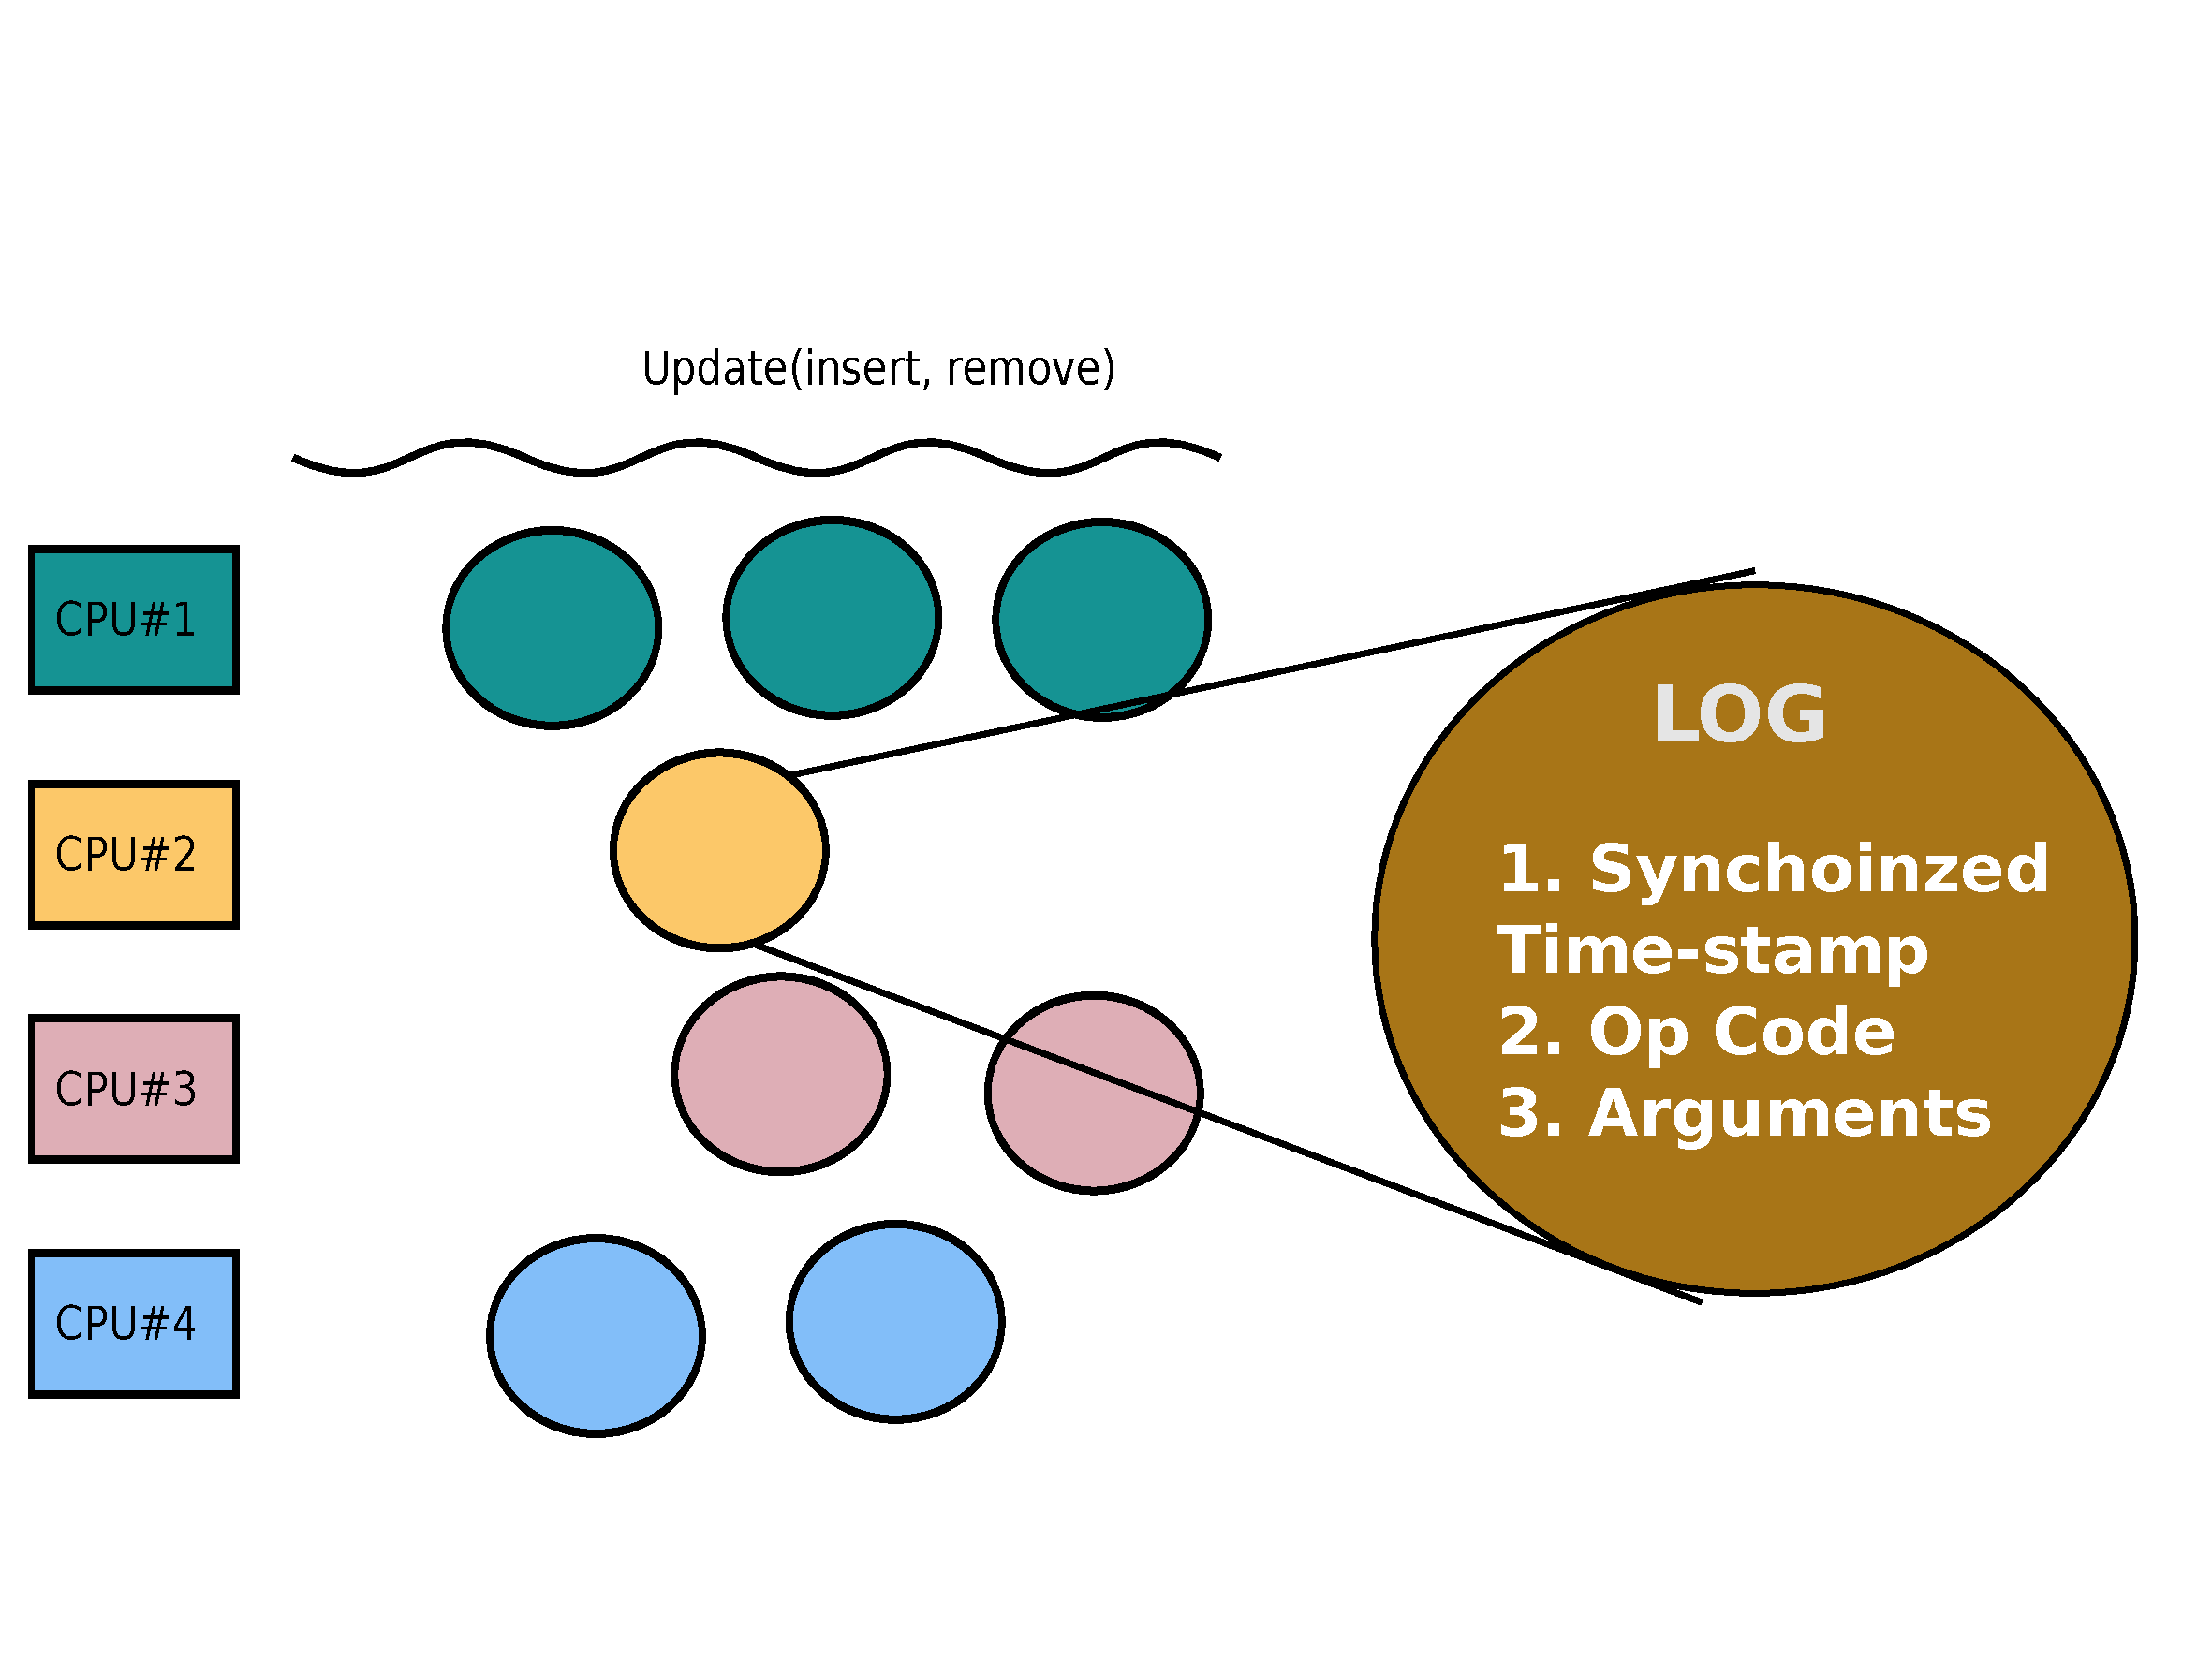
\includegraphics[width=0.8\textwidth]{fig/oplog_log}
    \caption{OpLog의 업데이트 방법}
  \label{fig:oplog}
\end{figure}



